\section{Cloudsysteme -- Funktionalität}
\label{sec:cloudfunktionalitaet}

\textbf{Was ändert sich in der Cloud?}
\begin{items}
	\item Physischer Entwurf muss automatisch erfolgen
	\item Obligatorische Datenverteilung
	\item Anfrageauswertung in Gegenwart anderer Anfragen
		\\*
		\( \leadsto \) entsprechende Planung
	\item Unterschiedliche QoS-Vereinbarungen mit unterschiedlichen Dienstnehmern
	\item Plötzliche extreme Zunahme von Zugriffen eines Dienstnehmers i.A. nicht vorhersehbar 
		\\*
		\( \leadsto \) Infrastruktur sollte damit umgehen können
	\item \emph{Secure Storage}: Verschlüsselung der Daten, trotzdem soll Dienstanbieter möglichst großen Teil der Anfrageauswertung übernehmen
\end{items}

\textbf{Relationale Algebra}
\begin{items}
	\item \underline{Projektion}: Optimierung: bei vielen Projektionen hintereinander reicht die zuletzt ausgeführte auch allein:
		\\*
		\( \pi \)\lstinline{[KName](}\( \pi \)\lstinline{[KName, Land](Kuenstler))} \( \leadsto \) \( \pi \)\lstinline{[KName](Kuenstler)}
	\item \underline{Selektion}: Optimierung: Selektionen lassen sich beliebig vertauschen, manchmal auch Projektion und Selektion
	\item \underline{Verbund}: Kommutativ, Assoziativ
		\\*
		Nested-Loop Join: Teuer, da pro Eintrag links über alle rechten Einträge iteriert wird
		\\*
		Merge Join: Beide Relationen sortieren, dann Eintrag für Eintrag
\end{items}

\textbf{Blockierende/Nichtblockierende Operatoren}
\begin{items}
	\item Operator blockiert \( \Leftrightarrow \) Ergebnis des Operators muss vor Ausführung des nachfolgenden vollständig berechnet sein \\* (z.B. Sort-Operator)
\end{items}

\textbf{Histogramme}
\begin{items}
	\item Zeigt Auftrittshäufigkeit eines Intervalls
	\item \underline{Equi-Width-Histogramm}: Breite aller Buckets gleich
	\item \underline{Equi-Depth-Histogramm}: Auftrittshäufigkeit aller Buckets gleich
	\item Nützlich bei ein-Attribut-Anfragen, sonst nicht so:
		\\*
		Mehrdimensionale Histogramme schwer konstruierbar und wartbar, Anzahl Attributkombinationen exponentiell wachsend zur Anzahl der Attribute
\end{items}

\textbf{Synchroner und asynchroner Zugriff}
\begin{items}
	\item \underline{Synchron}: innerhalb einer Transaktion
	\item \underline{Asynchron}: mehrere Transaktionen
\end{items}

\textbf{Service-Level Agreements}
\begin{items}
	\item Vereinbarung zwischen Client und Server bzgl. Dienstausführung
		\\*
		``Antwort innserhalb von 300ms für 99,9\% der Aufrufe bei 500 Zugriffen pro Sekunde''
\end{items}

\textbf{Zustände}
\begin{items}
	\item \underline{Zustandslos}: z.B. Umrechnungsdienst
	\item \underline{Zustandsbehaftet}: z.B. Ausführung Geschäftsprozess
\end{items}

\textbf{Quorum}
\begin{items}
	\item Szenario: Replikation mit \( n \) Knoten
		\\*
		\( \leadsto \) Wie Konsistenz sicherstellen? Was, wenn nicht alle Knoten verfügbar?
	\item \underline{Quorum Consensus}:
		\\*
		Lesen: Lese Mindestanzahl von Versionen (\( R \)), nehme aktuelle
		\\*
		Schreiben: Aktualisiere Mindestanzahl von Kopien (\( W \))
		\\*
		\( \leadsto \) Für Lesen/Schreiben muss eine festgelegte Anzahl an Knoten zustimmen. Forderungen (\( N \) = Anzahl Knoten):
		\begin{enumeration}
			\item \( Q_R+Q_W > N \)
			\item \( 2Q_W > N \)
		\end{enumeration}
\end{items}

\newpage

\textbf{P2P}
\begin{items}
	\item \emph{peer to peer}-Systeme:
		\\*
		Jeder Knoten für Ausschnitt des Schlüsselraums verantwortlich
		\\*
		Verwaltung von (Schlüssel, Wert)-Paaren
		\\*
		(put, get)-Interface
		\\*
		Zu Größe des Schlüsselraums logarithmischer Suchaufwand
	\item Beispiel: Chord
		\\*
		Zentrale Datenstruktur: \emph{identifier circle}, \emph{chord ring}
		\\* Suche: Jeder Knoten hat \emph{finger table}, \emph{i}-ter Eintrag von Knoten \( n \): successor(\( n+2^{i-1} \)) (\( m \) Anzahl Bits)
	\begin{figure}[H]\centering\label{Chord}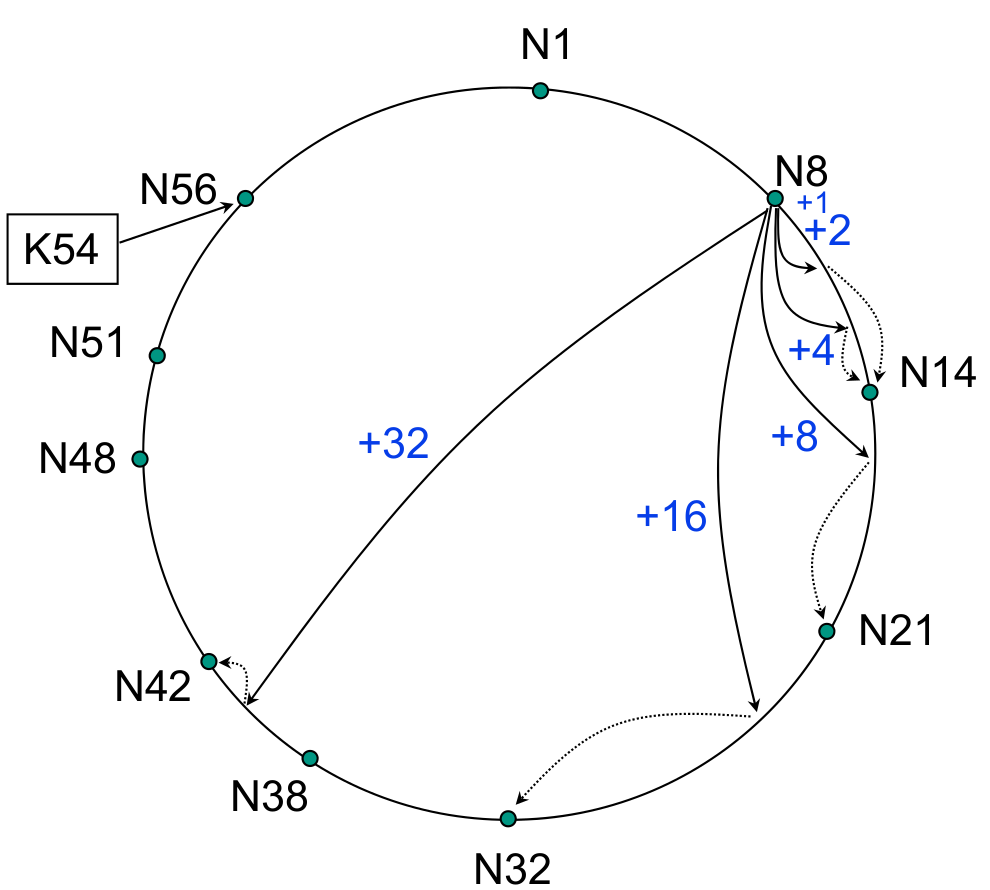
\includegraphics[width=0.25\textwidth]{Chord}\end{figure}
	\item Replikation über \emph{chained replication}: Schlüssel nicht nur bei einem Knoten, sondern auch bei \( k \) Nachfolgern einfügen
	\item \underline{Heterogenität}: Knoten können unterschiedlich leistungsstark sein (ggf. unterschiedliche Zuständigkeitsbereiche, unterschiedliche Last)
\end{items}

\textbf{Dynamo}
\begin{items}
	\item Key-Value-Store
	\item get-/put-Interface
	\item Objekte BLOBs \( \leadsto \) kein DB-Schema \( \leadsto \) Interpretieren nötig
	\item Keine Isolation \( \leadsto \) keine totale Konsistenz
	\item Schreibzugriff jeweils nur für ein Objekt
\end{items}
\begin{figure}[H]\centering\label{UebersichtDynamo}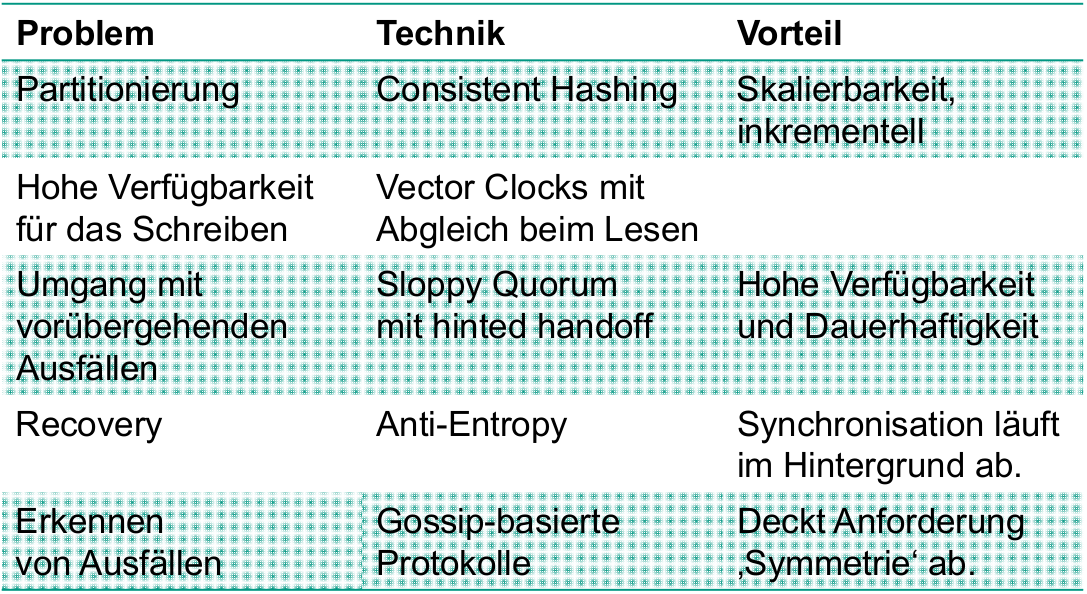
\includegraphics[width=0.33\textwidth]{UebersichtDynamo}\end{figure}

\textbf{Dynamo -- Vector Clocks}
\begin{items}
	\item Ziel: eventual consistency
	\item Liste von (Knoten, Zähler)-Paaren (eine Liste pro Version) \( \leadsto \) Erfassung der Zusammenhönge zwischen Versionen
	\item Quorum-basierte Techniken \( \leadsto \) Inkonsistenzen vermeiden
	\item vector clock-basierte Techniken \( \leadsto \) Inkonsistenzen erkennen und auflösen
	\item Unterschiedliche Knoten können Schreiboperationen absetzen \\* \( \leadsto \) Differenzierung
	\item Version 1 ist Vorgänger von Version 2, wenn jeder Zähler in List von V1 einen kleineren Wert hat als in der von V2
	\item Update (put) muss festlegen, welche Version aktualisiert werden soll
	\item Get gibt i.A. mehrere Versionen zurück
\end{items}

\newpage

\textbf{Scale Independence}
\begin{items}
	\item Anfrage ist \emph{scale-independent}
		\\*
		\( \leadsto \) Laufzeitverhalten unabhängig von DB-Größe
	\item Anfragenklassifikation nach Aufwand:
	\begin{enumeration}
		\item Klasse I (konstant):
			\\*
			z.B. ID-basierter Zugriff, \lstinline[language=sql]{LIMIT}-beschränkte Anfragen2
		\item Klasse II (beschränkt):
			\\*
			Explizite Begrenzung liegt vor
			\\*
			Als Kardinalität im erweiterten DB-Schema darstellbar
		\item Klasse III ((sub-)linear):
			\\*
			z.B. Ausgabe aller Kunden/Produkte
		\item Klasse IV (superlinear):
			\\*
			z.B. Clustering-Algo, der Self-Join der zugrundeliegenden Relation ausführt
	\end{enumeration}
	\item \( \leadsto \) \textbf{PIQL} (\emph{performance insightful query language}) - Scale Independent durch Erweiterungen und Beschränkungen der Anfragesprache
\end{items}

\textbf{Ergebnisgröße}
\begin{items}
	\item Wie bestimmte Größe des Anfrageergebnisses garantieren?
		\\*
		\( \leadsto \) \lstinline[language=sql]{LIMIT}, Pagination, Berücksichtigung von Fremdschlüsselbeziehungen, Erweiterung DB-Schema um Kardinalitäten
\end{items}

\textbf{Physische Optimierung}
\begin{items}
	\item Zwei Arten von physischen Operatoren:
	\begin{enumeration}
		\item \emph{remote operator}: Zugriffe auf key-value store und elementare Verarbeitungsschritte
		\item Client-seitige Operatoren für Query-Logik
	\end{enumeration}
	\item Remote Operator: Muss explizite Beschränkung der Größe des Zwischenergebnisses enthalten (i.A. \lstinline{stop}-Operator in Operator-Darstellung)
	\item Remote-Operatoren:
	\begin{enumeration}
		\item \textbf{IndexScan}: Prädikat muss zusammenhängendem Ausschnitt des indexierten Wertebereichs entsprechen, ``Sort'' muss Sortierreihenfolge des Index sein
		\item \textbf{IndexForeignKeyJoin}: Beschränkung durch Fremdschlüsseleigenschaft \( \leadsto \) kein logischer Stop-Operator, linker Teilausdruck enthält Fremdschlüssel
		\item \textbf{SortedIndexJoin}: Bei Sortierung des Inputs nach Join Key lässt sich aus limit hint-Begrenzuung der Anzahl an Datenobjekten pro Schlüssel ableiten
	\end{enumeration}
\end{items}

\textbf{SLO Compliance-Vorhersage}
\begin{items}
	\item SLO = \emph{serivce-level objectives}
	\item Größenbeschränkung Zwischenergebnisse noch keine Garantie für insgesamt beschränkten Aufwand
	\item Wenn anliegende Last sehr groß kann IndexScan-Ausführung beliebig lange dauern
	\item Lookup über Zufallsverteilung (Parameter Tupelgröße, Anzahl erwarteter Tupel)
\end{items}

\begin{fragen}
	\begin{enumeration}
		\item Was für Möglichkeiten kennen Sie, den Join zu implementieren? Weche Komplexität haben sie?
		\item Welche Möglichkeiten kennen Sie, den Aufwand, den eine Anfrage verursacht, zu reduzieren/begrenzen?
	\end{enumeration}
\end{fragen}